\subsection{Noether 环的 Hausdorff 完备化}

设 A 为交换环，m 为 A 的理想，E 为 A-模；令 \(\hat{A}\) 和 \(\hat{E}\) 分别表示 A 和 E 关于 m-进拓扑的 Hausdorff 完备化，\(j_{E}\) 表示典范映射 \(E \rightarrow \hat{E}\)。A-双线性映射 \((a, x) \mapsto aj_{\mathrm{E}}(x)\) 从 \(\hat{A} \times E\) 到 \(\hat{E}\)，定义了一个 A-线性映射

\[
\alpha_ {\mathrm{E}} \colon \hat {\mathrm{A}} \otimes_ {\mathrm{A}} \mathrm{E} \rightarrow \hat {\mathrm{E}},
\]

称为典范映射。设 \(u: \mathrm{E} \to \mathrm{F}\) 是 A-模同态，\(\hat{u}\colon \hat{\mathbf{E}}\to \hat{\mathbf{F}}\) 是由取 Hausdorff 完备化得到的映射；对于 \(a\in \hat{\mathbf{A}},x\in \mathbf{E},\)

\[
\alpha_ {\mathrm{F}} (a \otimes u (x)) = a j _ {\mathrm{F}} (u (x)) = a \hat {u} (j _ {\mathrm{E}} (x)) = \hat {u} (\alpha_ {\mathrm{E}} (a \otimes x)),
\]

换言之，图

\pandocbounded{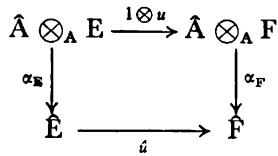
\includegraphics[keepaspectratio]{images/part002_24f0cc04.jpg}}

是交换的。最后，由第 2 节第 12 号命题 16 可知，若 E 有限生成，则同态 \(\alpha_{\mathbb{E}}\) 是满射。

定理 3。设 A 为交换 Noether 环，m 为 A 的理想，E、F、G 为三个有限生成的 A-模。则：

\begin{enumerate}
\def\labelenumi{(\roman{enumi})}
\item
  若 \(E \xrightarrow{u} F \xrightarrow{v} G\) 是 A-线性映射的正合列，则对 m-进拓扑取 Hausdorff 完备化所得的序列 \(\hat{E} \xrightarrow{\hat{u}} \hat{F} \xrightarrow{\hat{v}} \hat{G}\) 是正合的。
\item
  典范的 \(\hat{\mathbf{A}}\)-线性映射 \(\alpha_{\mathbf{E}}: \hat{\mathbf{A}} \otimes_{\mathbf{A}} \mathbf{E} \to \hat{\mathbf{E}}\) 是双射。
\item
  A-模 \(\hat{\mathbf{A}}\) 是平坦的。
\end{enumerate}

我们已经看到，u 和 v 是拓扑群的严格态射（第 2 号，定理 2 的推论）。断言 (i) 于是由第 2 节第 12 号引理 2 得出。当 E = A 时，断言 (ii) 显然成立；当 E 是有限生成自由 A-模时，立即可归约到此情形。一般地，E 有一个有限表示

\[
\mathrm{L} \xrightarrow {u} \mathrm{L} ^ {\prime} \xrightarrow {v} \mathrm{E} \longrightarrow 0
\]

（第一章，第 2 节，第 8 号，引理 8）。于是得到一个交换图

\pandocbounded{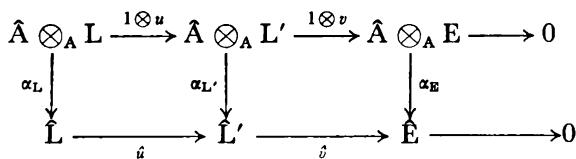
\includegraphics[keepaspectratio]{images/part002_14bc27b3.jpg}}

第一行是正合的（第一章，第 2 节，第 1 号，引理 1），由 (i) 第二行也正合。我们已经知道 \(\alpha_{\mathrm{E}}\) 是满射（第 2 节，第 12 号，命题 16）；另一方面，由于 \(\alpha_{\mathrm{L}}\) 和 \(\alpha_{\mathrm{L}'}\) 是双射且 \(1 \otimes v\) 是满射，根据第一章第 1 节第 4 号命题 2 的推论 2，\(\alpha_{\mathrm{E}}\) 是单射；这就证明了 (ii)。

由 (i) 和 (ii) 可知，若 \(a\) 是 \(A\) 的理想（必然有限生成），则典范映射 \(\hat{A} \otimes_{A} a \to \hat{A}\) 是单射，因为它是 \(\hat{a} \to \hat{A}\) 与 \(\alpha_{E}\) 的复合；这证明了 \(\hat{A}\) 是平坦的 A-模（第一章，第 2 节，第 3 号，命题 1）。

在定理 3 的条件下，\(\hat{\mathbf{A}}\otimes_{\mathbf{A}}\mathbf{E}\) 常识别为 \(\hat{\mathbf{E}}\)，借助典范映射 \(\alpha_{\mathbf{E}}\)。若 \(u\colon \mathbf{E}\to \mathbf{F}\) 是有限生成 A-模的同态，则由图（4）的交换性，\(\hat{u}\colon \hat{\mathbf{E}}\to \hat{\mathbf{F}}\) 识别为 \(1\otimes u\)。

推论 1。设 A 为交换 Noether 环，m 为 A 的理想，E 为有限生成的 A-模，F、G 为 E 的两个子模。赋予 A、E、F、G 以 m-进拓扑，令 i 为从 E 到 Ê 的典范映射。则：

\[
\begin{array}{r l} \hat {\mathbf {F}} = \hat {\mathbf {A}}. i (\mathbf {F}), & (\mathbf {F} + \mathbf {G}) ^ {\wedge} = \hat {\mathbf {F}} + \hat {\mathbf {G}}, \\ & (\mathbf {F} \cap \mathbf {G}) ^ {\wedge} = \hat {\mathbf {F}} \cap \hat {\mathbf {G}}, \\ & (\mathbf {F}: \mathbf {G}) ^ {\wedge} = \hat {\mathbf {F}}: \hat {\mathbf {G}}. \end{array}
\]

此外，若 a、b 是 A 的两个理想且 c = ab，则 \(\hat{c} = \hat{ab}\)。

根据定理 3，\(\hat{\mathbf{E}}\)、\(\hat{\mathbf{F}}\)、\(\hat{\mathbf{G}}\) 分别典范地识别为 \(\hat{\mathbf{A}} \otimes_{\mathbf{A}} \mathbf{E}\)、\(\hat{\mathbf{A}} \otimes_{\mathbf{A}} \mathbf{F}\)、\(\hat{\mathbf{A}} \otimes_{\mathbf{A}} \mathbf{G}\)，这就建立了前两个公式。第三个和第四个分别由第一章第 2 节第 6 号命题 6 及第 10 号命题 12 得出。最后，由于 \(\hat{\mathbf{a}} = \hat{\mathbf{A}}i(\mathfrak{a})\)、\(\hat{\mathfrak{b}} = \hat{\mathbf{A}}i(\mathfrak{b})\)、\(\hat{\mathfrak{c}} = \hat{\mathbf{A}}i(\mathfrak{c})\)，

\[
\hat {\mathfrak {c}} = \hat {\mathrm{A}} i (\mathfrak {a b}) = \hat {\mathrm{A}} i (\mathfrak {a}) i (\mathfrak {b}) = \hat {\mathfrak {a b}}.
\]

推论 2。设 A 为交换 Noether 环，m 为 A 的理想，\(\hat{\mathbf{A}}\) 为 A 关于 m-进拓扑的 Hausdorff 完备化。若元素 \(a \in \mathbf{A}\) 不是 A 中的零因子，则它的典范像 \(a'\) 在 \(\hat{\mathbf{A}}\) 中不是 \(\hat{\mathbf{A}}\) 中的零因子。

由于 \(\hat{\mathbf{A}}\) 是平坦的 A-模，该推论是第一章第 2 节第 4 号命题 3（i）的特殊情形。

推论 3。若 A 是交换 Noether 环，则形式幂级数环 A{[}{[}X₁, \ldots, Xₙ{]}{]} 是平坦的 A-模。

它是多项式环

\[
\mathbf {B} = \mathbf {A} [ \mathbf {X} _ {1}, \dots , \mathbf {X} _ {n} ]
\]

关于 m-进拓扑，其中 m 是不含常数项的多项式组成的集合（第 2 节，第 12 号，例 1）；由于 B 是 Noether 环（第 2 节，第 10 号，定理 2 的推论 2），根据定理 3，A{[}{[}X₁, \ldots, Xₙ{]}{]} 是平坦的 B-模；又由于 B 是自由 A-模，A{[}{[}X₁, \ldots, Xₙ{]}{]} 是平坦的 A-模（第一章，第 2 节，第 7 号，命题 8 的推论 3）。

命题 8。设 A 为交换 Noether 环，m 为 A 的理想，\(\hat{A}\) 为 A 关于 m-进拓扑的 Hausdorff 完备化，j 为从 A 到 \(\hat{A}\) 的典范映射。则：

\begin{enumerate}
\def\labelenumi{(\roman{enumi})}
\item
  \(\hat{\mathbf{A}}\) 是 Zariski 环，且 \(\hat{\mathfrak{m}} = \hat{\mathbf{A}}.j(\mathfrak{m})\) 是 \(\hat{\mathbf{A}}\) 的定义理想。
\item
  映射 \(\mathfrak{n} \mapsto \hat{\mathfrak{n}} = \hat{\mathbf{A}}.j(\mathfrak{n})\) 将 \(\mathbf{A}\) 中包含 \(\mathfrak{m}\) 的极大理想集双射到 \(\hat{\mathbf{A}}\) 的极大理想集，而 \(\mathfrak{q} \mapsto j^{-1}(\mathfrak{q})\) 是其逆双射。
\item
  设 \(\mathfrak{n}\) 是 \(\mathbf{A}\) 的包含 \(\mathfrak{m}\) 的极大理想。同态 \(j': \mathbf{A}_{\mathfrak{n}} \to \hat{\mathbf{A}}_{\hat{\mathfrak{n}}}\) 由 \(j\) 得到且是单射；若将 \(\mathbf{A}_{\mathfrak{n}}\) 通过 \(j\) 识别为 \(\hat{\mathbf{A}}_{\hat{\mathfrak{n}}}\) 的子环，则 \((\mathfrak{n}\mathbf{A}_{\mathfrak{n}})\)-进拓扑在 \(\mathbf{A}_{\mathfrak{n}}\) 上由 \(\hat{\mathfrak{n}}\)-进拓扑在 \(\hat{\mathbf{A}}_{\hat{\mathfrak{n}}}\) 上诱导，且 \(\mathbf{A}_{\mathfrak{n}}\) 在 \(\hat{\mathbf{A}}_{\hat{\mathfrak{n}}}\) 中关于 \(\hat{\mathfrak{n}}\)-进拓扑稠密。
\end{enumerate}

证明 (i)。由于 \(\mathfrak{m}\) 是有限生成的理想，\((\mathfrak{m}^n)^{\circ} = (\hat{\mathfrak{m}})^n = \mathfrak{m}^n\hat{\mathbf{A}}\)（第 2 节，第 12 号，命题 16 的推论 2），且 \(\hat{\mathbf{A}}\) 上的拓扑是 \(\hat{\mathfrak{m}}\)-进拓扑。由于 \(\hat{\mathbf{A}}/\hat{\mathfrak{m}}\) 同构于 \(\mathbf{A}/\mathfrak{m}\)，它是 Noether 环，而 \(\hat{\mathfrak{m}} = \mathfrak{m}\hat{\mathbf{A}}\) 是有限生成的 \(\hat{\mathbf{A}}\)-模，因而 \(\hat{\mathbf{A}}\) 是 Noether 环（第 2 节，第 10 号，定理 2 的推论 5）；最后，由于 \(\hat{\mathbf{A}}\) 关于 \(\hat{\mathfrak{m}}\)-进拓扑是 Hausdorff 且完备的，\(\hat{\mathbf{A}}\) 是 Zariski 环（第 3 号，例 1）。

断言 (ii) 立即由以下事实得出：由 j 得到的典范同态 \(A/m \rightarrow \hat{A}/\hat{m}\) 是双射，并且 \(\hat{A}\) 的每个极大理想都包含 \(\hat{m}\)，因为 \(\hat{A}\) 是 Zariski 环，故 \(\hat{A}\) 的 Jacobson 根包含 \(\hat{m}\)（第 3 号，命题 6）。

最后证明 (iii)。由于 \(\mathfrak{n} = j^{-1}(\hat{\mathfrak{n}}), j(\mathbf{A} - \mathfrak{n}) \subset \hat{\mathbf{A}} - \hat{\mathfrak{n}}\)，\(j\) 确实定义了同态 \(j' \colon \mathbf{A}_{\mathfrak{n}} \to \hat{\mathbf{A}}_{\hat{\mathfrak{n}}}\)（第二章，第 2 节，第 1 号，命题 2）。证明 \(j'\) 是单射；设 \(a \in \mathbf{A}, s \in \mathbf{A} - \mathfrak{n}\)，满足

\[
j ^ {\prime} (a / s) = j (a) / j (s) = 0;
\]

则存在 \(s' \in \hat{\mathbf{A}} - \hat{\mathfrak{n}}\)，使得 \(s'j(a) = 0\)（第二章，第 2 节，第 1 号，注 3），所以 \(j(a)\) 在 \(\hat{\mathbf{A}}\) 中的湮没子不包含于 \(\hat{\mathfrak{n}}\)。现在，若 \(\mathfrak{b}\) 是 \(a\) 在 \(\mathbf{A}\) 中的湮没子，则 \(j(a)\) 在 \(\hat{\mathbf{A}}\) 中的湮没子为 \(\mathfrak{b}\)（定理 3 的推论 1）；因而 \(\mathfrak{b} \not\subset \mathfrak{n}\)，这表明 \(a / s = 0\)。

此外，还有一个交换图

\[
\begin{array}{c} \mathrm{A} / \mathfrak {n} ^ {k} \longrightarrow \mathrm{A} _ {\mathfrak {n}} / (\mathfrak {n} \mathrm{A} _ {\mathfrak {n}}) ^ {k} \\ \stackrel {{h}} {{\downarrow}} \qquad \qquad \qquad \qquad \qquad \qquad \qquad \qquad \qquad \qquad \qquad \qquad \qquad \qquad \qquad \qquad \qquad \qquad \qquad \qquad \qquad \qquad \qquad \hat {\mathrm{A}} / \hat {\mathfrak {n}} ^ {k} \longrightarrow \hat {\mathrm{A}} _ {\hat {\mathfrak {n}}} / (\hat {\mathfrak {n}} \hat {\mathrm{A}} _ {\hat {\mathfrak {n}}}) ^ {k} \end{array}\tag{5}
\]

其中 \(h\) 和 \(h'\) 分别由 \(j\) 和 \(j'\) 得到，水平箭头是第二章第 3 节第 3 号命题 9 的典范同构。由于 \(n^k\) 是 A 的开理想（因为它包含 \(m^k\)），\(h\) 是双射，因而 \(h'\) 也是双射。这首先表明 \((\mathfrak{n}\mathbf{A}_{\mathfrak{n}})^k = j'((\hat{\mathfrak{n}}\hat{\mathbf{A}}_{\hat{\mathfrak{n}}})^k)\)，因而 \(\mathbf{A}_{\mathfrak{n}}\) 上的拓扑由 \(\hat{\mathbf{A}}_{\hat{\mathfrak{n}}}\) 上的拓扑诱导；此外，\(\hat{\mathbf{A}}_{\hat{\mathfrak{n}}} = \mathbf{A}_{\mathfrak{n}} + (\hat{\mathfrak{n}}\hat{\mathbf{A}}_{\hat{\mathfrak{n}}})^k\) 对所有 \(k > 0\) 都成立，因而 \(\mathbf{A}_{\mathfrak{n}}\) 在 \(\hat{\mathbf{A}}_{\hat{\mathfrak{n}}}\) 中处处稠密。

推论。设 A 为 Noether 局部环（分别为半局部环），m 为其 Jacobson 根。则 \(\hat{A}\) 是 Noether 局部环（分别为半局部环），其 Jacobson 根为 \(\hat{m}\)。

\(\hat{\mathbf{A}}\) 根据命题 8（i）是 Noether 环，其余结论由命题 8（ii）及定理 3 的推论 1 中的第三个公式得出。

